\documentclass[11pt]{article}
\usepackage[utf8]{inputenc}
\usepackage[italian]{babel}
\usepackage[margin = 1in]{geometry}
\usepackage{amsfonts, amsmath, amssymb}

\usepackage{fancyhdr}
\usepackage{graphicx}
\usepackage{float}
\usepackage{ulem}

\pagestyle{fancy}
\fancyhead{}
\fancyfoot{}
\fancyhead [L]{\slshape \MakeUppercase{Local volatility model 2018/2019}}
\fancyfoot[C]{\thepage}

\begin{document}
\begin{titlepage}
\begin{center}
\vspace*{1cm}
\Large{Politecnico di Milano}
\vfill
\line(1,0){400}\\[1mm]
\huge{\textbf{Modello di Volatilità Locale\\}}
\vspace*{1cm}
\Large{\textbf{Progetto per l'A.A. 2018/2019}}\\[1mm]
\line(1,0){400}\\
\vfill
\textbf{Autori:}\\
Laura Locatelli\\
Pietro Manzoni\\
Matteo Paggiaro\\
Luca Parafioriti\\
\vspace*{2cm}
14 Gennaio 2019
\end{center}
\end{titlepage}

\section{Ottimizzazione del codice}

Per prima cosa, procediamo alla stesura della funzione richiesta. Notiamo che all'interno del codice \texttt{example\_calibration\_ecorp.m} fornitoci a lezione è già presente una funzione \texttt{solve\_dupire.m}. In realtà la struttura complessiva è più articolata e prevede una chiamata a cascata di più funzioni annidate:
\
\begin{equation*}
	\texttt{example\_calibration\_ecorp.m} \rightarrow
	\texttt{calibrator.m} \rightarrow
	\texttt{model\_volatility.m}\rightarrow
	\texttt{solve\_dupire.m}
\end{equation*}

Decidiamo così di ritoccare le ultime due, allegate al progetto con i nomi \texttt{model\_volatility\_mod.m} e \texttt{solve\_dupire\_mod.m}. Nello specifico, le maggiori modifiche apportate riguardano proprio quest'ultima: la funzione originale \texttt{solve\_dupire.m} riceve in ingresso un tempo di expiry $T_1$ (oltre a molti altri dati e parametri) e risolve numericamente l'equazione di Dupire nella regione $[k_{min},k_{max}]\times[0,T_1]$. Tuttavia, durante il processo di calibrazione del modello, si rende necessario calcolare la soluzione per diverse expiries $\{T_1, T_2\dots, T_N\}$: qui il codice mostra tutta la sua inefficienza, andando a risolvere ogni volta l'equazione nell'intera regione $[k_{min},k_{max}]\times[0,T_k]$, quando invece la soluzione è già nota in $[k_{min},k_{max}]\times[0,T_{k-1}]$ dall'iterazione precedente.\\

Invece, per quanto riguarda la funzione \texttt{model\_volatility\_mod.m}, le modifiche sono puramente teniche (e non concettuali) per via del fatto che l'output di \texttt{solve\_dupire\_mod.m} è ora in forma matriciale e non più vettoriale.\\

Completa infine il trittico la funzione \texttt{calibrator\_mod.m}, che si differenzia da \texttt{calibrator.m} per il semplice fatto di chiamare \texttt{model\_volatility\_mod.m} al posto di \texttt{model\_volatility.m}.\\

Da ultimo, ci teniamo a sottolineare due piccole cose:

\begin{itemize}
	\item[$\rhd$] poichè tipicamente le expiries non sono equamente distribuite, la griglia che viene creata da \texttt{solve\_dupire\_mod.m} non è più equispaziata. Infatti il passo di discretizzazione temporale nell'intervallo $[T_{k-1},T_k]$ è tanto più raffinato quanto più le due scadenze sono vicine nel tempo. Tuttavia riteniamo che ciò non sia assolutamente un problema in termini di affidabilità o cattiva approssimazione della soluzione.

	\item[$\rhd$] il codice originale \texttt{solve\_dupire.m} mantiene in ogni caso la propria utilità nei casi in cui sia necessario risolvere l'equazione di Dupire per un'unica data di expiry, come si osserverà al punto successivo.
\end{itemize}

\vfill
\section{ECORP}

\subsection{Calibrazione dei dati}
Consideriamo adesso i dati di mercato estratti dal dataset \texttt{ECORP}.\\
Utilizzando il codice ottimizzato \texttt{calibrator\_mod.m} sviluppato nell'esercizio precedente, calibriamo il modello con il comando:\\

\texttt{[V] = calibrator\_mod(T,Knorm,MktVol,tol,MaxIter, N,M,Kmin, Kmax, 'cn');}\\

La funzione restituisce la matrice \texttt{V}, legata alla volatilità $\eta(t,x)$ del modello attraverso la relazione:

\begin{equation}
V_{ij} = \eta(T_i,K_{ij})
\end{equation}

Il grafico dell'errore di approssimazione mostra come la calibrazione faccia sì che la volatilità del modello coincida con quella del mercato.

\begin{figure}[H]
\centering
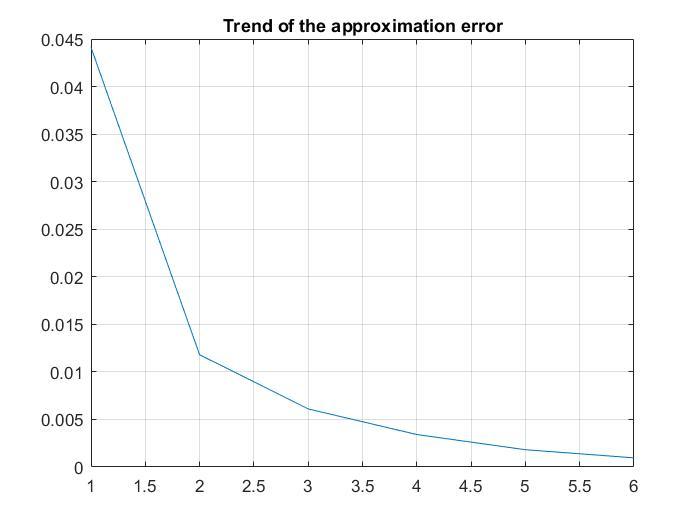
\includegraphics[width=0.5\textwidth]{cal}
\end{figure}

\subsection{Pricing di opzioni Call}
Si vuole adesso calcolare il prezzo di due Call Option (EU) con Maturity $T=0.5$ anni e Strike $K_1 = 0.9 S(0)$ e $K_2 = 1.1S(0)$.\\
Ottenuta la volatilità $\eta(t,x)$ del modello attraverso la calibrazione precedente, è possibile calcolare i prezzi delle call attraverso la risoluzione numerica dell'\textbf{equazione di Dupire}:
\begin{equation}
\frac{\partial}{\partial T}c_0(T,k) = \frac{1}{2}\eta^2(T,k)k^2\frac{\partial^2}{\partial k^2}c_0(T,k)
\end{equation} 
\vspace*{1cm}
L'equazione di Dupire lega così $\eta(t,x)$ ai prezzi delle call normalizzate. La risoluzione numerica dell'equazione viene affidata alla function \texttt{solve\_dupire.m} già implementata.\\
Attraverso la relazione $$C_0(T,K) = D_0(T)F_0(T)c_0(T,k)$$ 
si possono poi riscalare i prezzi calcolati, ottenendo:
\begin{align*}
C_0(T,K_1) &= 286.6985 & \sigma^{BS}(T,K_1) &= 11.93\%\\
C_0(T,K_2) &= 4.3049 & \sigma^{BS}(T,K_2) &= 8.31
\end{align*}

Inoltre, per completezza, decidiamo di implementare una simulazione con il metodo di Monte Carlo in modo da ottenere un'approssimazione del prezzo delle due call options. Per quanto questo approccio stocastico porti ogni volta ad un risultato numerico diverso, lanciando qualche volta il codice si può apprezzare come i valori ottenuti tendano ad essere ragionevolmente vicini ai prezzi calcolati. 
 

\subsection{Simulazione di Monte Carlo}
\paragraph{Forward Starting Options}
Una forward starting option con date $T_1$ e $T_2 > T_1$ è un opzione con payoff dato da:
\begin{equation}
\Phi(T_1,T_2) = (S(T_2)-kS(T_1))^+
\end{equation}
con $k>0$. Il prezzo dell'opzione all'istante $T_1$ è dato da:
\begin{equation}
C_{T_1}(T_1,T_2,k)= D_{T_1}(T_2)\mathbb{E}[\Phi(T_1,T_2)|\mathcal{F}_{T1}]
\end{equation}

\paragraph{Pricing}
Anche nella sezione 2.3 del codice \texttt{point2.m} viene eseguita una simulazione di Monte Carlo per stimare i prezzi di due forward options aventi $T_1 = 2$, $T_2 = 2.5$ e $k_1=0.9$, $k_2=1.1$.\\
Otteniamo quindi:
\begin{align*}
C_{T_1}(T_1,T_2,k_1) &= 298.12 & \sigma^{BS}_{fwd}(T_1,T_2,k_1) &= 16.53\%\\
C_{T_1}(T_1,T_2,k_2) &= 32.77 & \sigma^{BS}_{fwd}(T_1,T_2,k_2) &= 15.15\%\\
\end{align*}

\subsection{Volatility smile}
Utilizzando la calibrazione del modello fatta nel punto 2.1, otteniamo le due curve spot e forward della volatilità:

\begin{figure}[H]
\centering
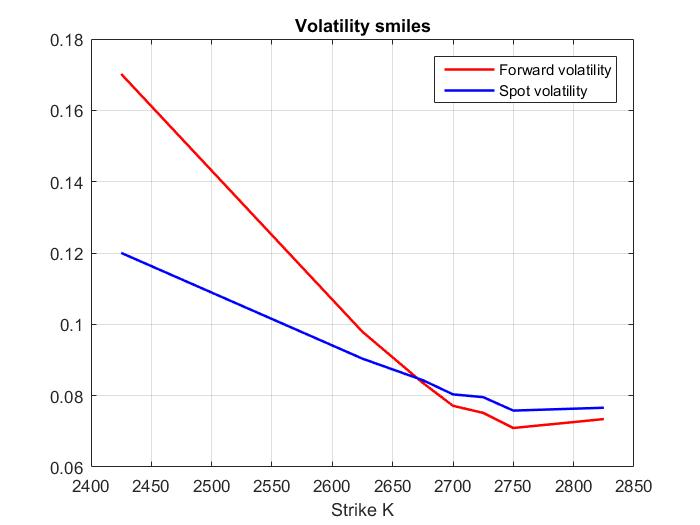
\includegraphics[width=0.5\textwidth]{vol_smile}
\end{figure}

Il grafico evidenzia una caratteristica tipica del Modello di Volatilità Locale, ossia il fatto che la curva della volatilità forward abbia una pendenza maggiore di quella spot.

\subsection{La caduta dei giganti}

A questo punto della trattazione, supponiamo di scoprire che in realtà la forward starting option di cui ci siamo appena occupati esiste veramente. Con trepidazione andiamo a controllare la sua quotazione e ci accorgiamo che è del tutto differente dal prezzo che abbiamo calcolato. Dovevamo e/o potevamo aspettarcelo?\\

In questo breve paragrafo daremo spazio ad alcune riflessioni riguardanti l'affidabilità e la verosimiglianza del \textit{Local Volatility Model}.\\

Per cominciare, ragioniamo sull'origine stessa del modello. Esso nasce come una modifica del modello Black and Scholes, nel tentativo di ovviare, probabilmente, a quella che è la più grande e pretenziosa ipotesi: l'introduzione di un parametro di volatilità costante. Ciò che era stata la fortuna di Black and Scholes -grazie al fatto di poter offrire delle formule chiuse per il pricing- ne aveva al contempo decretato l'inutilità pratica, dal momento che gli andamenti del mercato erano tutto fuorchè aderenti a ciò che era previsto da tale modello. Pertanto l'introduzione di una \textit{volatility surface} sembra a primo impatto essere decisamente un buon compromesso. D'altra parte un'analisi critica suggerisce che anche il \textit{Local Volatility Model} abbia i propri limiti strutturali.\\

Più nel dettaglio, ci siamo soffermati su tre aspetti che a nostro parere rappresentano i punti deboli del modello:

\begin{itemize}
	\item[$\rhd$] come spesso capita in queste situazioni, si cerca di estrapolare informazioni partendo da un set finito di dati. Nel nostro caso, abbiamo fatto largo uso di interpolazione (lineare e con spline) per risalire ai dati mancanti e, per quanto inevitabile, ciò è tipicamente fonte di errore.
	\item[$\rhd$] la necessità matematica di ricorrere al caso. Allo stesso modo infatti, anche l'utilizzo del metodo Monte Carlo ha luci e ombre. Si tratta sicuramente di un algoritmo semplice e facilmente applicabile ai nostri problemi, tuttavia l'aleatorietà del metodo non garantisce per nulla accuratezza nei risultati.
	\item[$\rhd$] infine, uno dei punti cruciali di questo modello (come di moltissimi altri), è il tentativo di spiegare completamente i prezzi dei titoli tramite la loro volatilità. Nonostante infatti l'intuizione e l'evidenza empirica suggeriscano che ci sia grande interdipendenza tra le due cose, non ci si può aspettare di avere una completa correlazione.
\end{itemize}



\section{FAIL}
Consideriamo adesso i dati presenti nelle tabelle \texttt{FAIL}. Utilizziamo, come in precedenza, il comando per la calibrazione del modello.\\ L'algoritmo non produce nessun risultato e restituisce un messaggio di errore.
Analizzando i grafici delle Volatilità Di Mercato in funzione delle Strikes Normalizzate, si osserva che nel caso della call con maturity 18 Dicembre stranamente non si ottiene una funzione convessa. 

\begin{figure}[H]
\centering
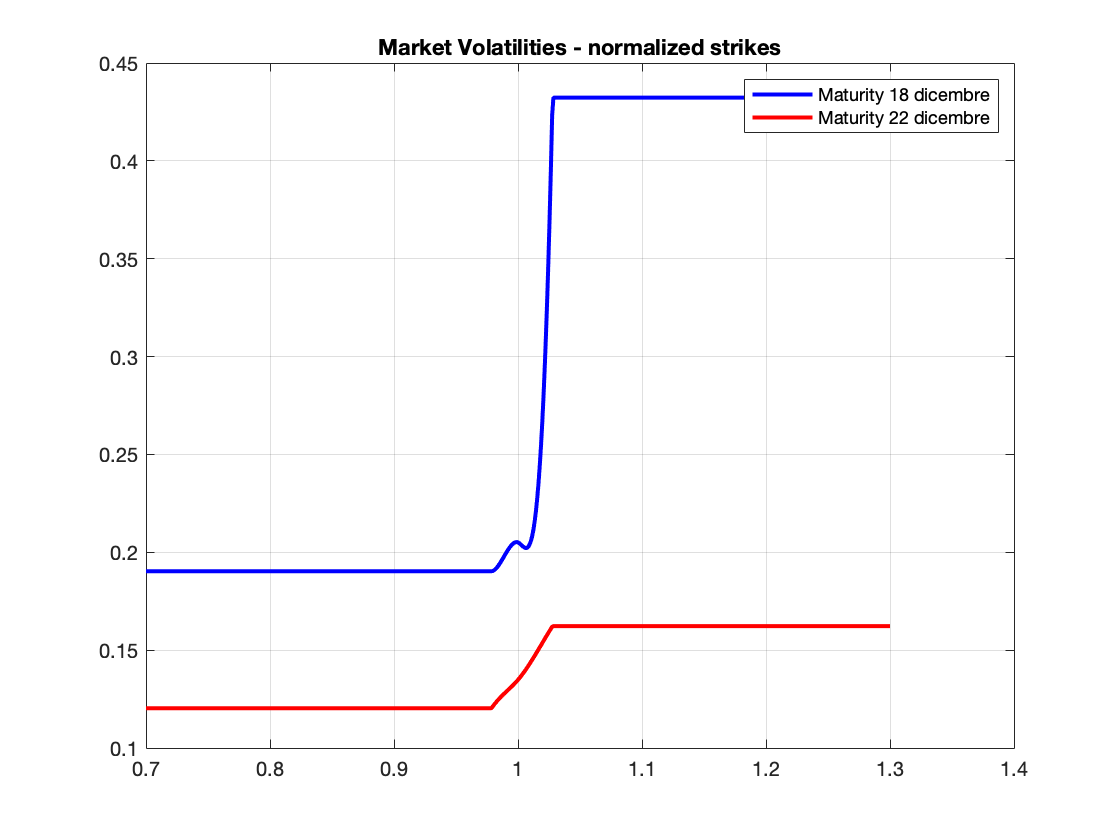
\includegraphics[width=0.5\textwidth]{MktVol_Knorm}
\end{figure}

L’anomalia per quest’ultima call si ripropone nell’analisi del prezzo delle Call in relazione alle Strikes, ove il suo grafico non presenta andamento decrescente (come invece avviene per la call con maturity 22 dicembre). 


\begin{figure}[H]
\centering
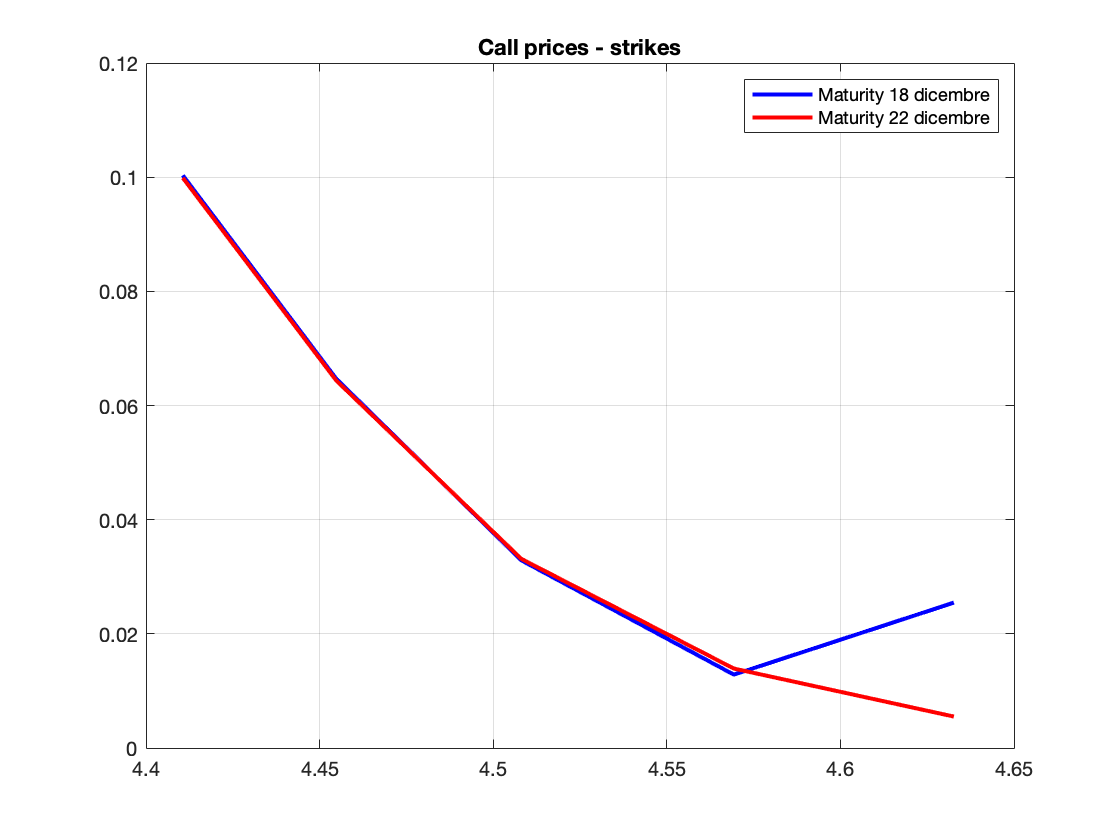
\includegraphics[width=0.5\textwidth]{C_K}
\end{figure}

Quest’ultima osservazione mette in luce un’opportunità di \textbf{arbitraggio}.\\
\paragraph{Costruzione dell'arbitraggio} Consideriamo i valori delle stikes $k_1=4.5693 < k_2=4.6327$, con i relativi prezzi della call con maturity 18 dicembre: $C(k_1)=0.0129 < C(k_2)=0.0255$. \\
\begin{itemize}


\item \textbf{$t=0$}: adottiamo una \textit{long position}  nella call con stike $k_1$ e una \textit{short position} nella call con strike $k_2$, investendo la differenza $C(k_2)-C(k_1)$ in banca.\\ In questo modo abbiamo un flusso netto di denaro pari a $$-C(k_1)+C(k_2)-(C(k_2)-C(k_1))=0$$

\item \textbf{$t=T$}: si registra un flusso di denaro pari a $$(S(T) – k_1)^+ - (S(T) – k_2)^+ + (C(k_2)-C(k_1))e^{rT}> 0 $$ poichè $k_1<k_2$ e $C(k_1)<C(k_2)$. 
\end{itemize}

Abbiamo quindi costruito un arbitraggio, tramite una strategia che senza alcun rischio comporta un portafoglio il cui valore iniziale è nullo, mentre alla maturity è sicuramente positivo.\\
Il dataset FAIL non rispetta quindi l’ipotesi di non-arbitraggio del modello teorico adottato; questo spiega il conseguente fallimento dell’algoritmo numerico.

\section{EURUSD}
Analizziamo adesso i dati di mercato dei tassi di cambio presenti nel database \texttt{EURUSD}. 

\subsection{Calibrazione del modello}
In generale le opzioni sui tassi di cambio non sono caratterizzate dagli Strike Price
ma dal $\Delta$, ovvero dalla sensibilità di Call Option EU scritte sui tassi rispetto ad una variazione di prezzo dei tassi stessi, definita nel modello Black \& Scholes come:
\begin{equation}
\Delta = \frac{\partial C_t(T)}{\partial X_t} = \mathcal{N}(d_1)
\end{equation}

Esiste un legame biunivoco tra $\Delta$ e gli strike $K$. Il parametro $d_1$ dipende infatti dallo strike $K$:

\begin{equation}
d_1(K) = \frac{\log\frac{F_0(T)}{K}+ \frac{\sigma(T,\Delta)}{2}}{\sigma(T,\Delta)\sqrt{T}}
\end{equation}

Otteniamo quindi il valore degli strike $\{ K_{ij}\}$ in funzione di $\{ T_i\}$ e $\{ \Delta_j\}$ risolvendo numericamente l'equazione $$\mathcal{N}(d_1(K)) = \Delta$$

Calcolati i valori degli strike prices procediamo poi con la calibrazione del modello, utilizzando ancora una volta la function \texttt{calibrator\_mod.m}.

\subsection{Modifica dello spot price}

Ci chiediamo adesso cosa succede se modifichiamo lo spot price:
$$ Y'(0) = 1.01\times Y(0)$$

Ricalcolando i prezzi aggiornati dei forward e stimando $K$ con la stessa procedura di prima, abbiamo tutti i parametri che servono per calibrare il modello. Otteniamo le seguenti curve di volatilità per i due differenti casi di spot.\\

\begin{figure}[H]
\centering
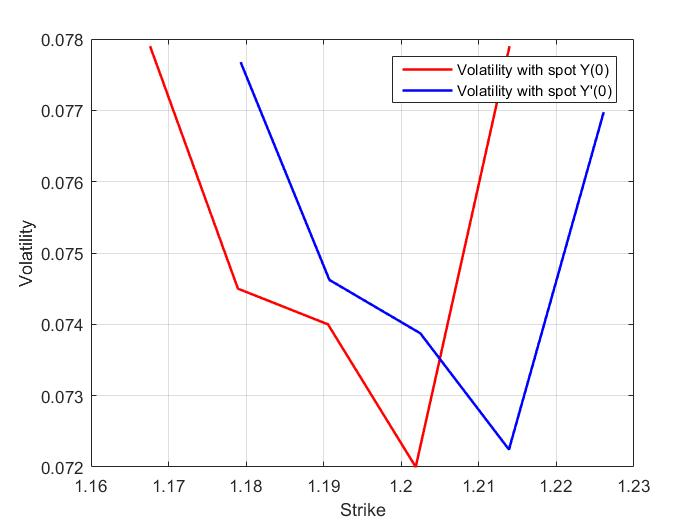
\includegraphics[width=0.5\textwidth]{sticky_delta}
\end{figure}
Dal grafico si evince che il modello si comporta come \textit{sticky-delta}. Si vede infatti come, al variare dello spot, la superficie di volatilità trasli in direzione del nuovo spot, mostrando quindi la sua dipendenza dal $\Delta$ e non dallo strike.


\end{document}